\documentclass[12pt,a4paper]{article}
\usepackage[utf8]{inputenc}
\usepackage[english]{babel}
\usepackage{amsmath}
\usepackage{amsfonts}
\usepackage{amssymb}
\usepackage{makeidx}
\usepackage{graphicx}
\usepackage{lmodern}
\usepackage{kpfonts}
\usepackage{tikz}
\usepackage{hyperref}
\usepackage[left=2cm,right=2cm,top=4cm,bottom=2cm]{geometry}
\setlength{\parindent}{0px}
\author{Daniel Vázquez Lago}
\title{Oscilaciones acopladas}

\begin{document}

\maketitle

\newpage

\tableofcontents

\newpage

\section{Objetivos}

Está práctica consta de los siguientes objetivos:

\begin{itemize}
\item Estudiar el movimiento de 2 masas unidas mediante diferentes muelles, y como podemos generalizarlo en función de las constantes de recuperación de los muelles (probando diferentes muelles), diferentes masas... En particular estudiaremos los movimientos normales de las masas y buscaremos las frecuencias de resonancia de estos modos (una de ellas).

\item Realizar el mismo estudio pero con 3 masas. En este caso no variaremos los muelles ni las masas, será un estudio mas cualitativo, simplemente buscando los modos normales.
\end{itemize}

\section{Análisis de datos}
\subsection{Calculo de constantes de recuperación}
En este caso estudiaremos la constante de recuperación de dos muelles que llamaremos ``muelle 1'' y ``muelle 2'' con $k_1$ y $k_2$  respectivamente. Calcularemos ambas mediante dos métodos: el método dinámico y estático. 

\begin{equation}
\text{Estático:} \ \Delta x = \dfrac{1}{k} g m ;  \ \ \text{Dinamico:} \ \dfrac{T^2}{4 \pi^2} = \dfrac{1}{k} m 
\end{equation} 

Teniendo en cuenta que $b=\dfrac{1}{k}$ podemos obtener k haciendo las regresiones lineales:


\begin{table}[h!] \centering 
\begin{tabular}{|c|c|c|c|}  
\hline 
$k_1$ (N/m) 	 & s($k_1$) (N/m) 	 & $k_2$ (N/m) 	 & s($k_2$) (n/m) \\ \hline  
3.17 	 & 0.12  	 & 2.287   	 & 0.067 \\ \hline 
\end{tabular} 
\caption{valores de las constantes de lo muelles} 
\label{tab:constantes-muelles} 
\end{table}


\begin{figure}[h!] \centering
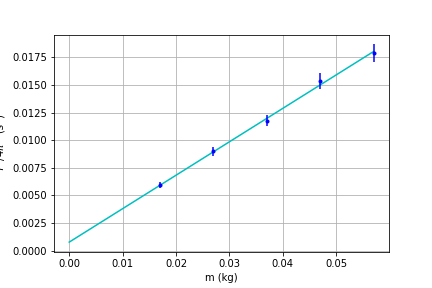
\includegraphics[scale=0.7]{plot1.png}
\end{figure}

\begin{figure}[h!] \centering
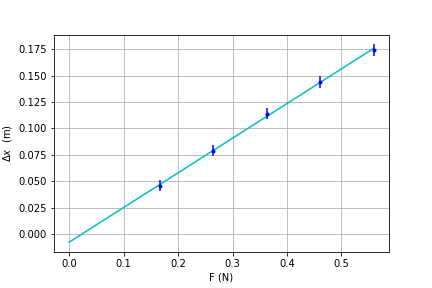
\includegraphics[scale=0.68]{plot2.png}
\end{figure}

\newpage

Para el muelle 2:

\begin{figure}[h!] \centering
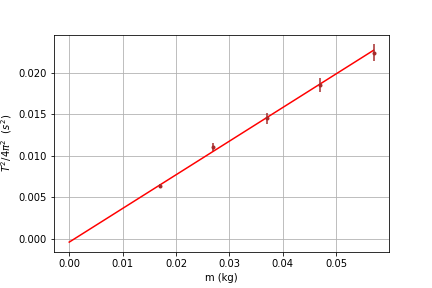
\includegraphics[scale=0.68]{plot3.png}
\end{figure}

\begin{figure}[h!] \centering
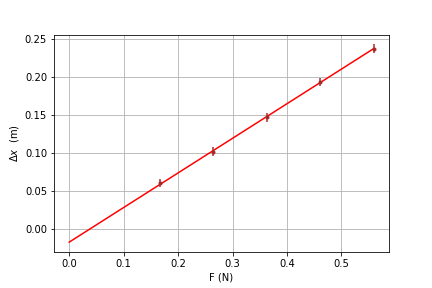
\includegraphics[scale=0.68]{plot4.png}
\end{figure}


\newpage

\subsection{Modos normales con 2 masas}
Como en este caso las partículas no se pueden mover en el eje z (condición que imponemos) el sistema tiene 4 grados de libertad (2 masas con 2 coordenadas generalizadas). Entonces podremos obtener hasta 4 modos normales (tras imponerle condiciones de contorno). Los diferentes modos normales están dibujados en la figura \ref{fig:modos-normales-2-masas}, siendo:
\begin{itemize}
\item \textbf{1):} modo normal simétrico. En este modo unidimensional la longitud del muelle central no varia como se refleja en la imagen. Vista frontal.
\item \textbf{2):} modo normal antisimétrico. En este modo unidimensional varían los 3 muelles, pero el centro del muelle central no varia (si las masas iguales este centro se encuentra en la mitad del muelle, si las masas no son iguales puede cambiar de posición, pero siempre va a haber una zona que no se mueva). Vista frontal.
\item \textbf{3):} modo normal trasversal simétrico. En este modo bidimensional el muelle del centro no varia de longitud. Vista en planta. 
\item  \textbf{4):} modo normal trasversal antisimétrico. En este modo bidimensinal, al igual que en el 2), hay un punto del muelle central que no se mueve. Vista en planta.
\end{itemize}


\begin{figure}[h!] \centering
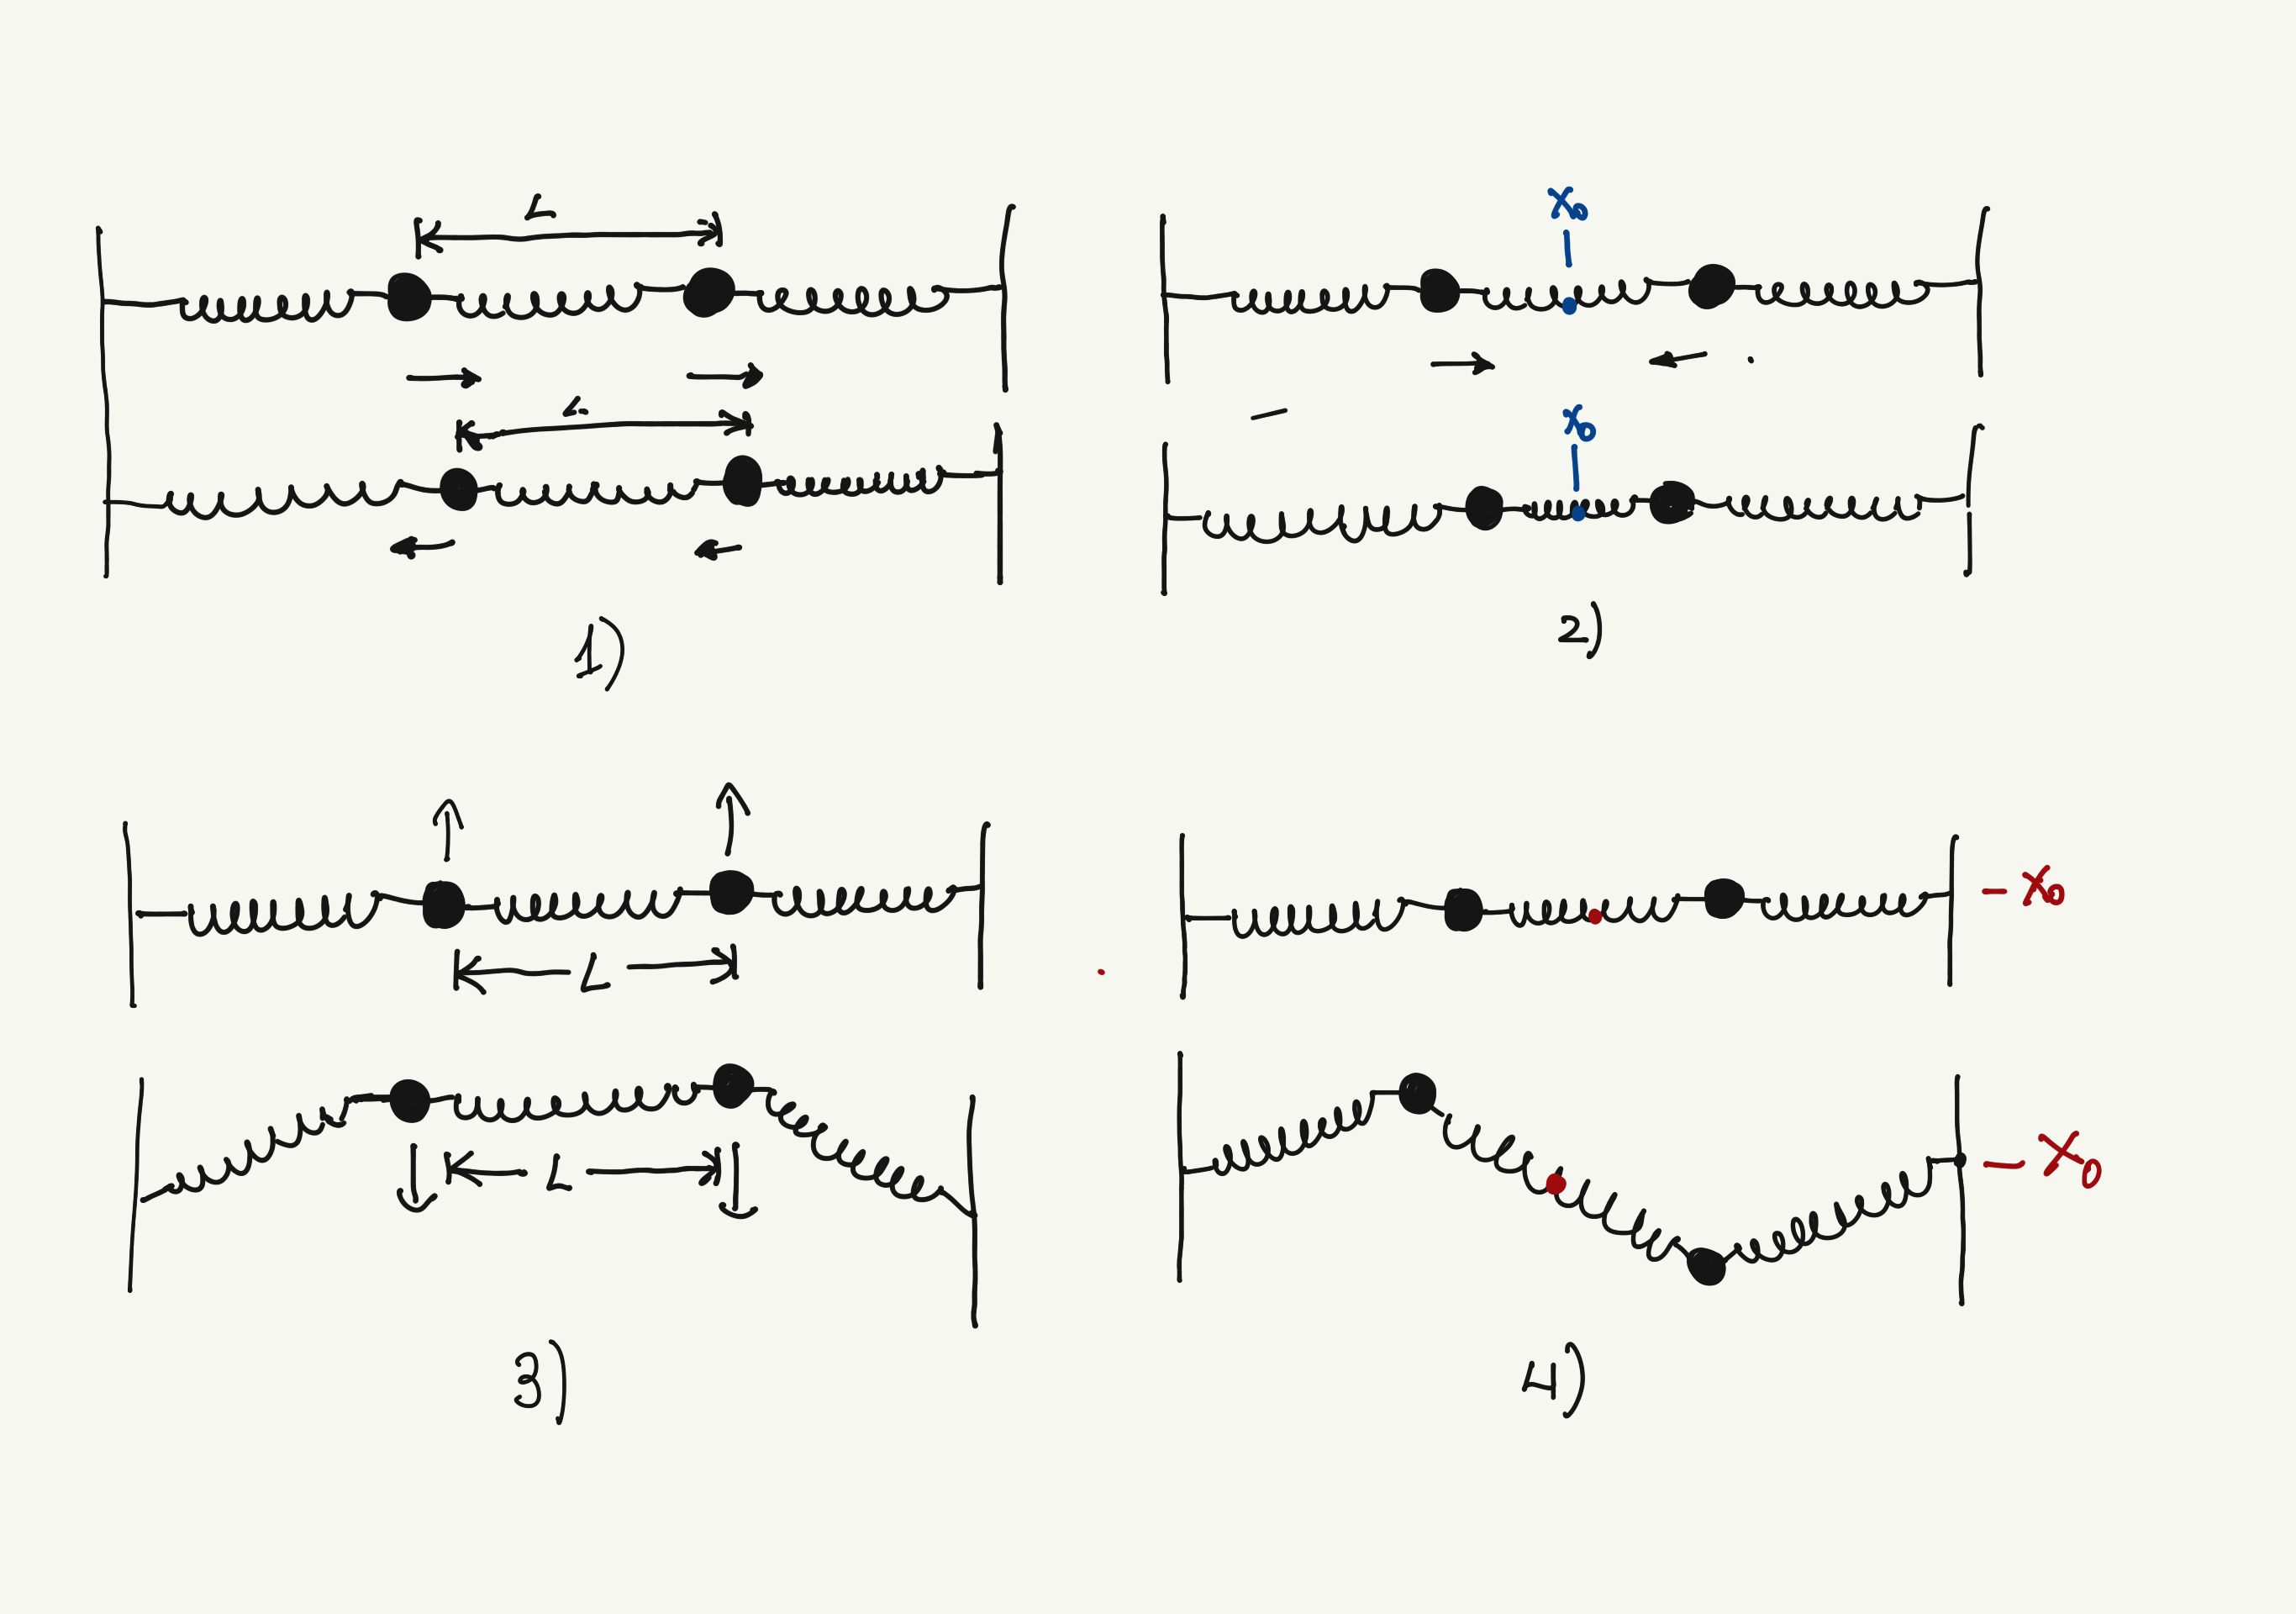
\includegraphics[scale=0.3]{Modo-normal-1.png}
\caption{modos normales de 2 masas unidas mediante muelles}
\label{fig:modos-normales-2-masas}
\end{figure}


En función de las masas y el muelle central que colocamos pudimos encontrar diferentes frecuencias de resonancia, tanto teóricas como experimentales. En las siguientes tablas representaremos las frecuencias de resonancia para cada modo, la teórica, y la experimental, en función de la constante de recuperación del muelle central y la masas colgadas. Cabe destacar que la constante de los muelles laterales los consideraremos iguales a $k_1$. Después compararemos las amplitudes relativas para cada caso. \\

\begin{table}[h!] \centering 
\begin{tabular}{|c|c|c|c|c|}  
\hline 
 	 & $f_T$ 	 & s($f_T$) 	 & $f_E$ 	 & s($f_E$) \\ \hline 
1) 	 & 0.896 	 & 0.014  	 & 0.909   	 & 0.001 \\
2) 	 & 1.552     & 0.041   	 & 1.542   	 & 0.001 \\
3) 	 &   -  	 &    -  	 & 0.775   	 & 0.030 \\
4) 	 &   -  	 &    -  	 & 1.285   	 & 0.083 \\
\hline 
\end{tabular} 
\caption{frecuencias (hz) con dos masas de 100g y muelle central de constante $k_1$}
\label{} 
\end{table}



\begin{table}[h!] \centering 
\begin{tabular}{|c|c|c|c|c|}  
\hline
 	 & $f_T$ 	 & s($f_T$) 	 & $f_E$ 	 & s($f_E$) \\ \hline
1) 	 & 0.896 	 & 0.029   	 & 0.935   	 & 0.001 \\ 
 2) 	 & 1.400 	 & 0.014 	 & 1.427   	 & 0.001 \\ 
 3) 	 &   -  	 &    -  	 & 0.856   	 & 0.007 \\ 
4) 	 &   -  	 &    -  	 & 1.138   	 & 0.013 \\ 
\hline
\end{tabular} 
\caption{frecuencias (hz) con dos masas de 100 g y muelle central de constante $k_2$}
\label{} 
\end{table}



\begin{table}[h!] \centering 
\begin{tabular}{|c|c|c|c|c|}  
\hline 
 	 & $f_T$ 	 & s($f_T$) 	 & $f_E$ 	 & s($f_E$) \\ \hline
1) 	 & 0.714 	 & 0.022  	 & 0.772   	 & 0.001 \\ 
2) 	 & 1.379	     & 0.061  	 & 1.310   	 & 0.001 \\ 
\hline 
\end{tabular} 
\caption{frecuencias (hz) con dos masas de 100g y 200g y  muelle central $k_1$}
\label{} 
\end{table}


\begin{table}[h!] \centering 
\begin{tabular}{|c|c|c|c|}  
\hline
 	 & $A_T$  	 & $A_E$ 	 & s($A_E$) \\ \hline 
1) 	 & 1   	 & 1.08      & 0.23 \\ 
 2) 	 & -1   	 & -1.00   	 & 0.47 \\ 
 \hline 
\end{tabular} 
\caption{amplitudes relativas para dos masas de 100g y el muelle central $k_1$}
\label{} 
\end{table}

\begin{table}[h!] \centering 
\begin{tabular}{|c|c|c|c|}  
\hline
 	 & $A_T$  	 & $A_E$ 	 & s($A_E$) \\ \hline 
1) 	 & 1   	 & 1.15   	 & 0.24 \\ 
 2) 	 & -1   	 & -0.80   	 & 0.26 \\ 
 \hline 
\end{tabular} 
\caption{amplitudes relativas para dos masas de 100g y el muelle central $k_2$}
\label{} 
\end{table}

\begin{table}[h!] \centering 
\begin{tabular}{|c|c|c|c|}  
\hline
 	 & $A_T$  	 & $A_E$ 	 & s($A_E$) \\ \hline 
1) 	 & 1.37   	 & 1.60   	 & 0.38 \\ 
 2) 	 & -0.37   	 & -0.71   	 & 0.35 \\ 
 \hline 
\end{tabular} 
\caption{amplitudes relativas para dos masas de 100g y 200g con el muelle $k_2$}
\label{} 
\end{table}

\newpage

\subsection{Modos normales con 3 masas}

En este caso tenemos 3 masas con 6 grados de libertad (3 masas con 2 coordenadas generalizadas cada una) entonces podremos hallar hasta 6 modos normales. Estos serán:



\begin{figure}[h!] \centering
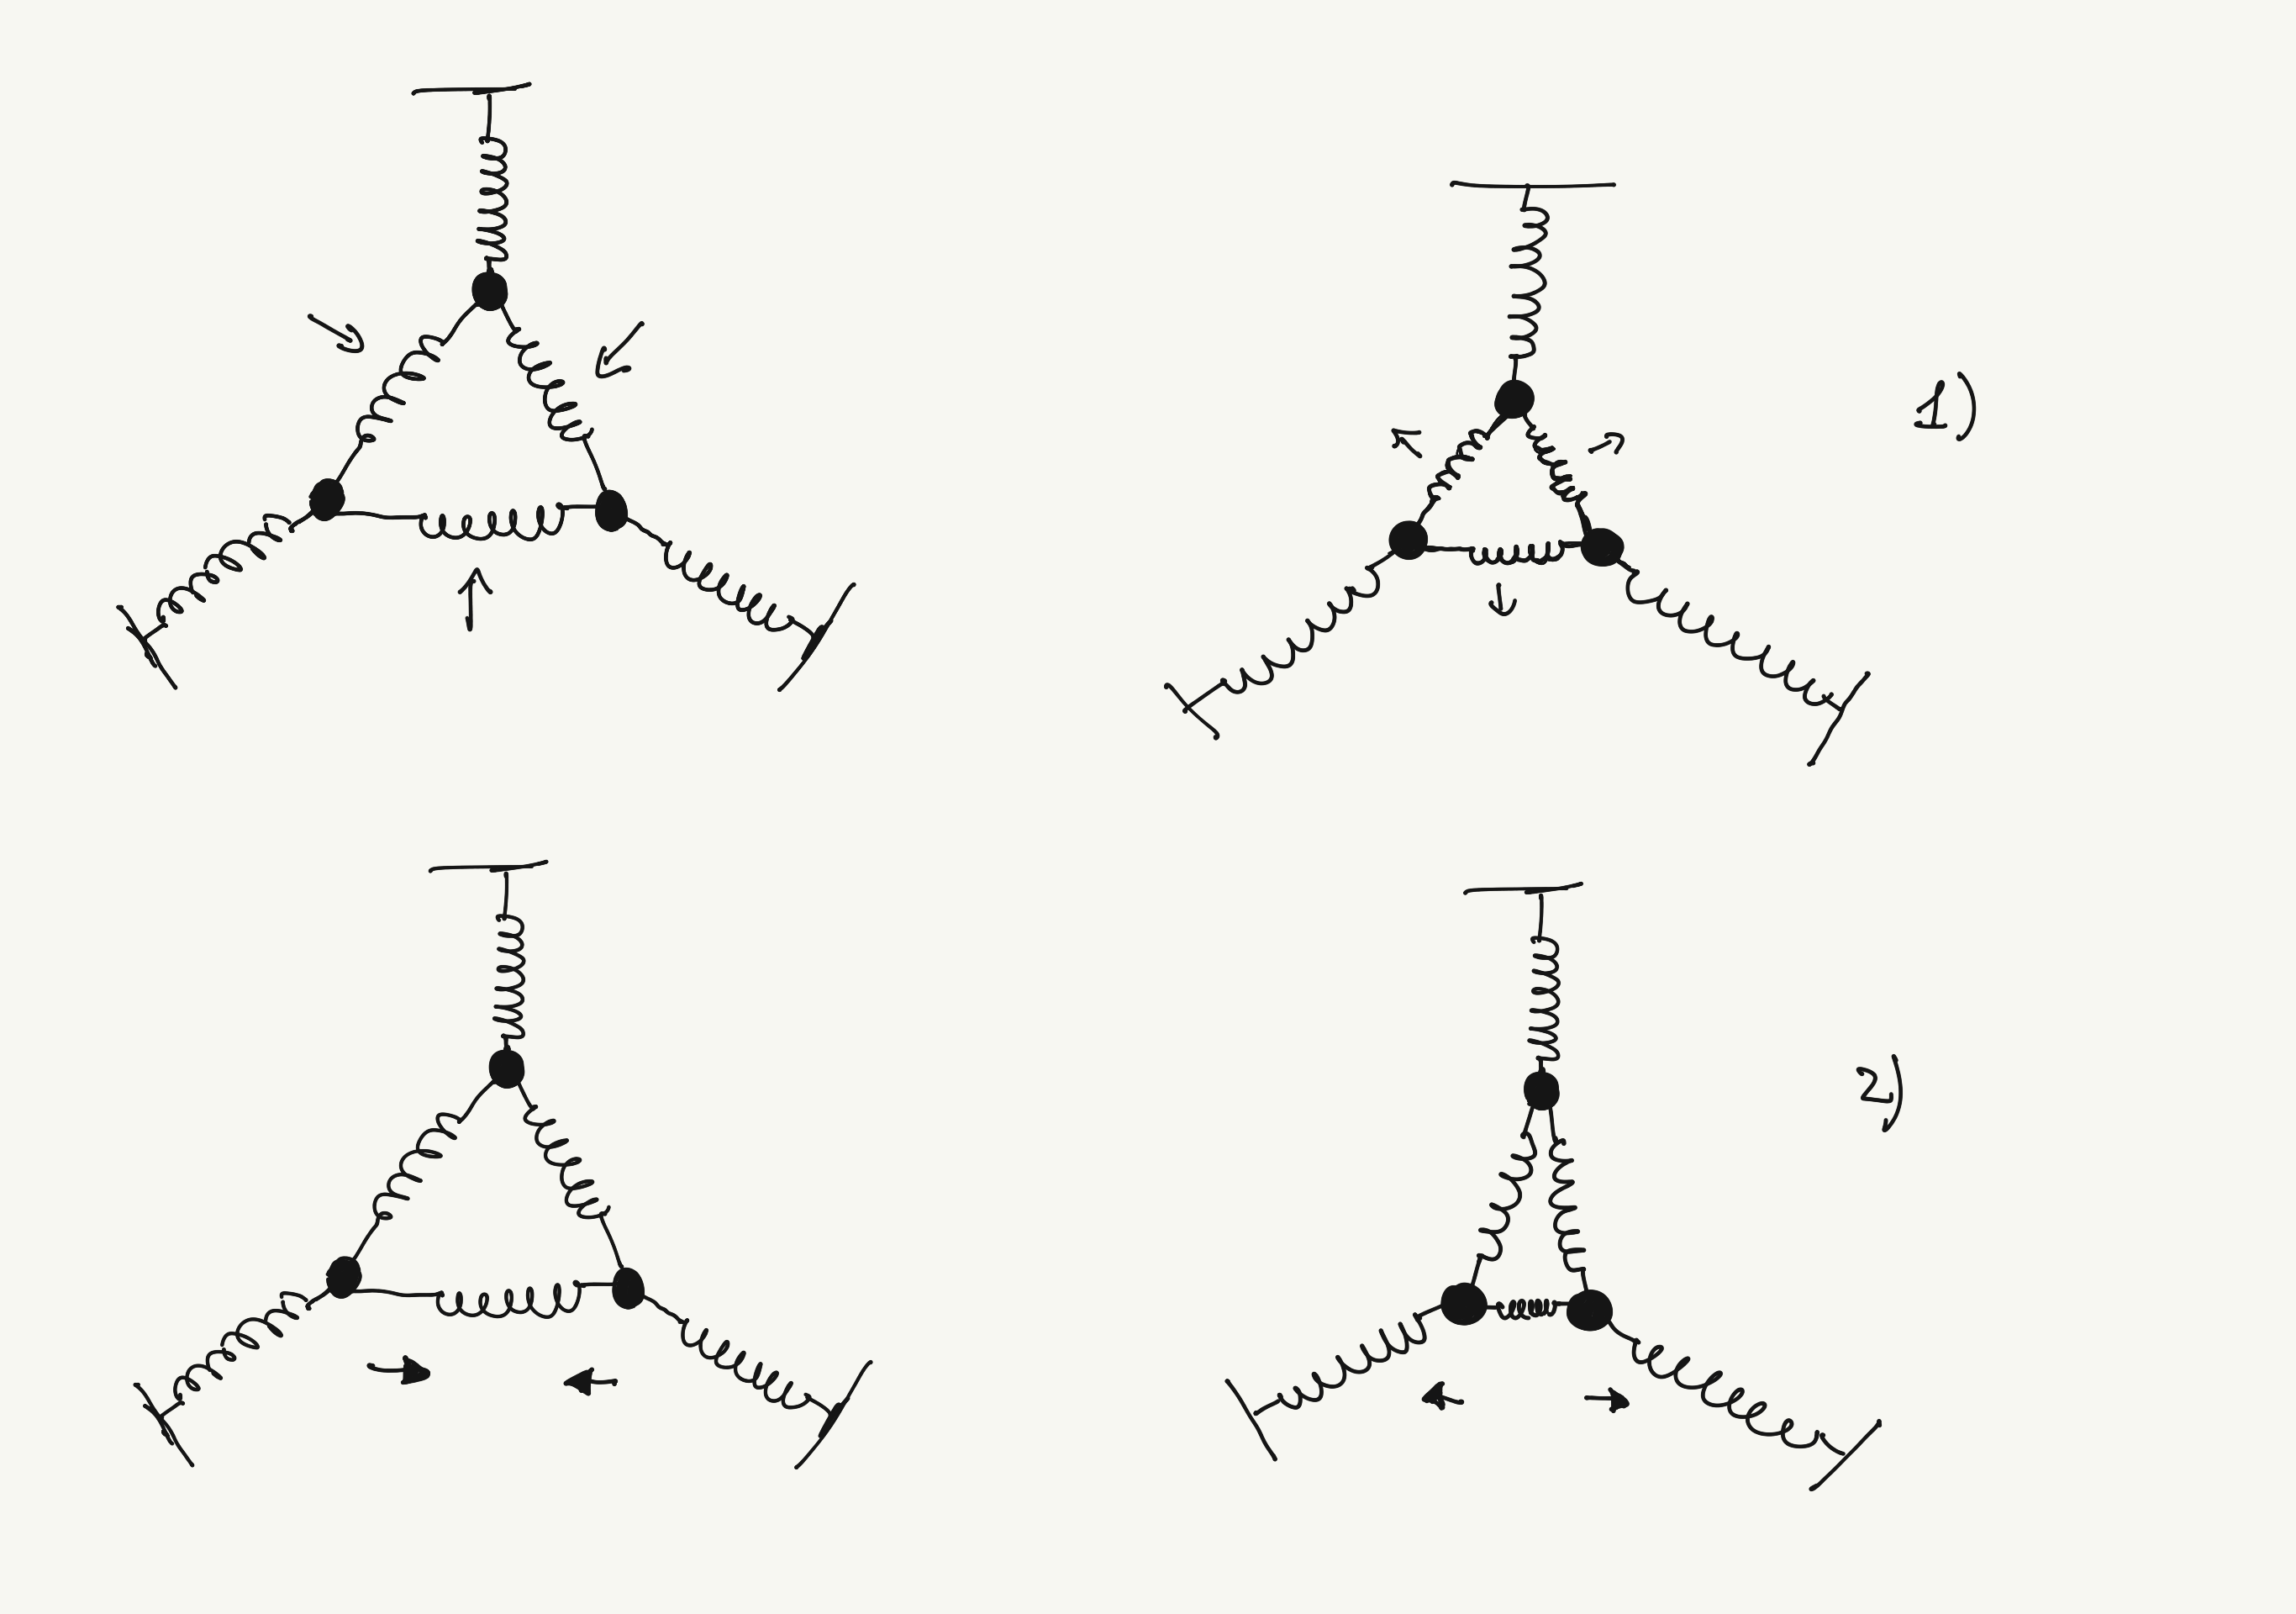
\includegraphics[scale=0.3]{Modo-normal-2.png}
\label{fig:1}
\end{figure}

\begin{figure}[h!] \centering
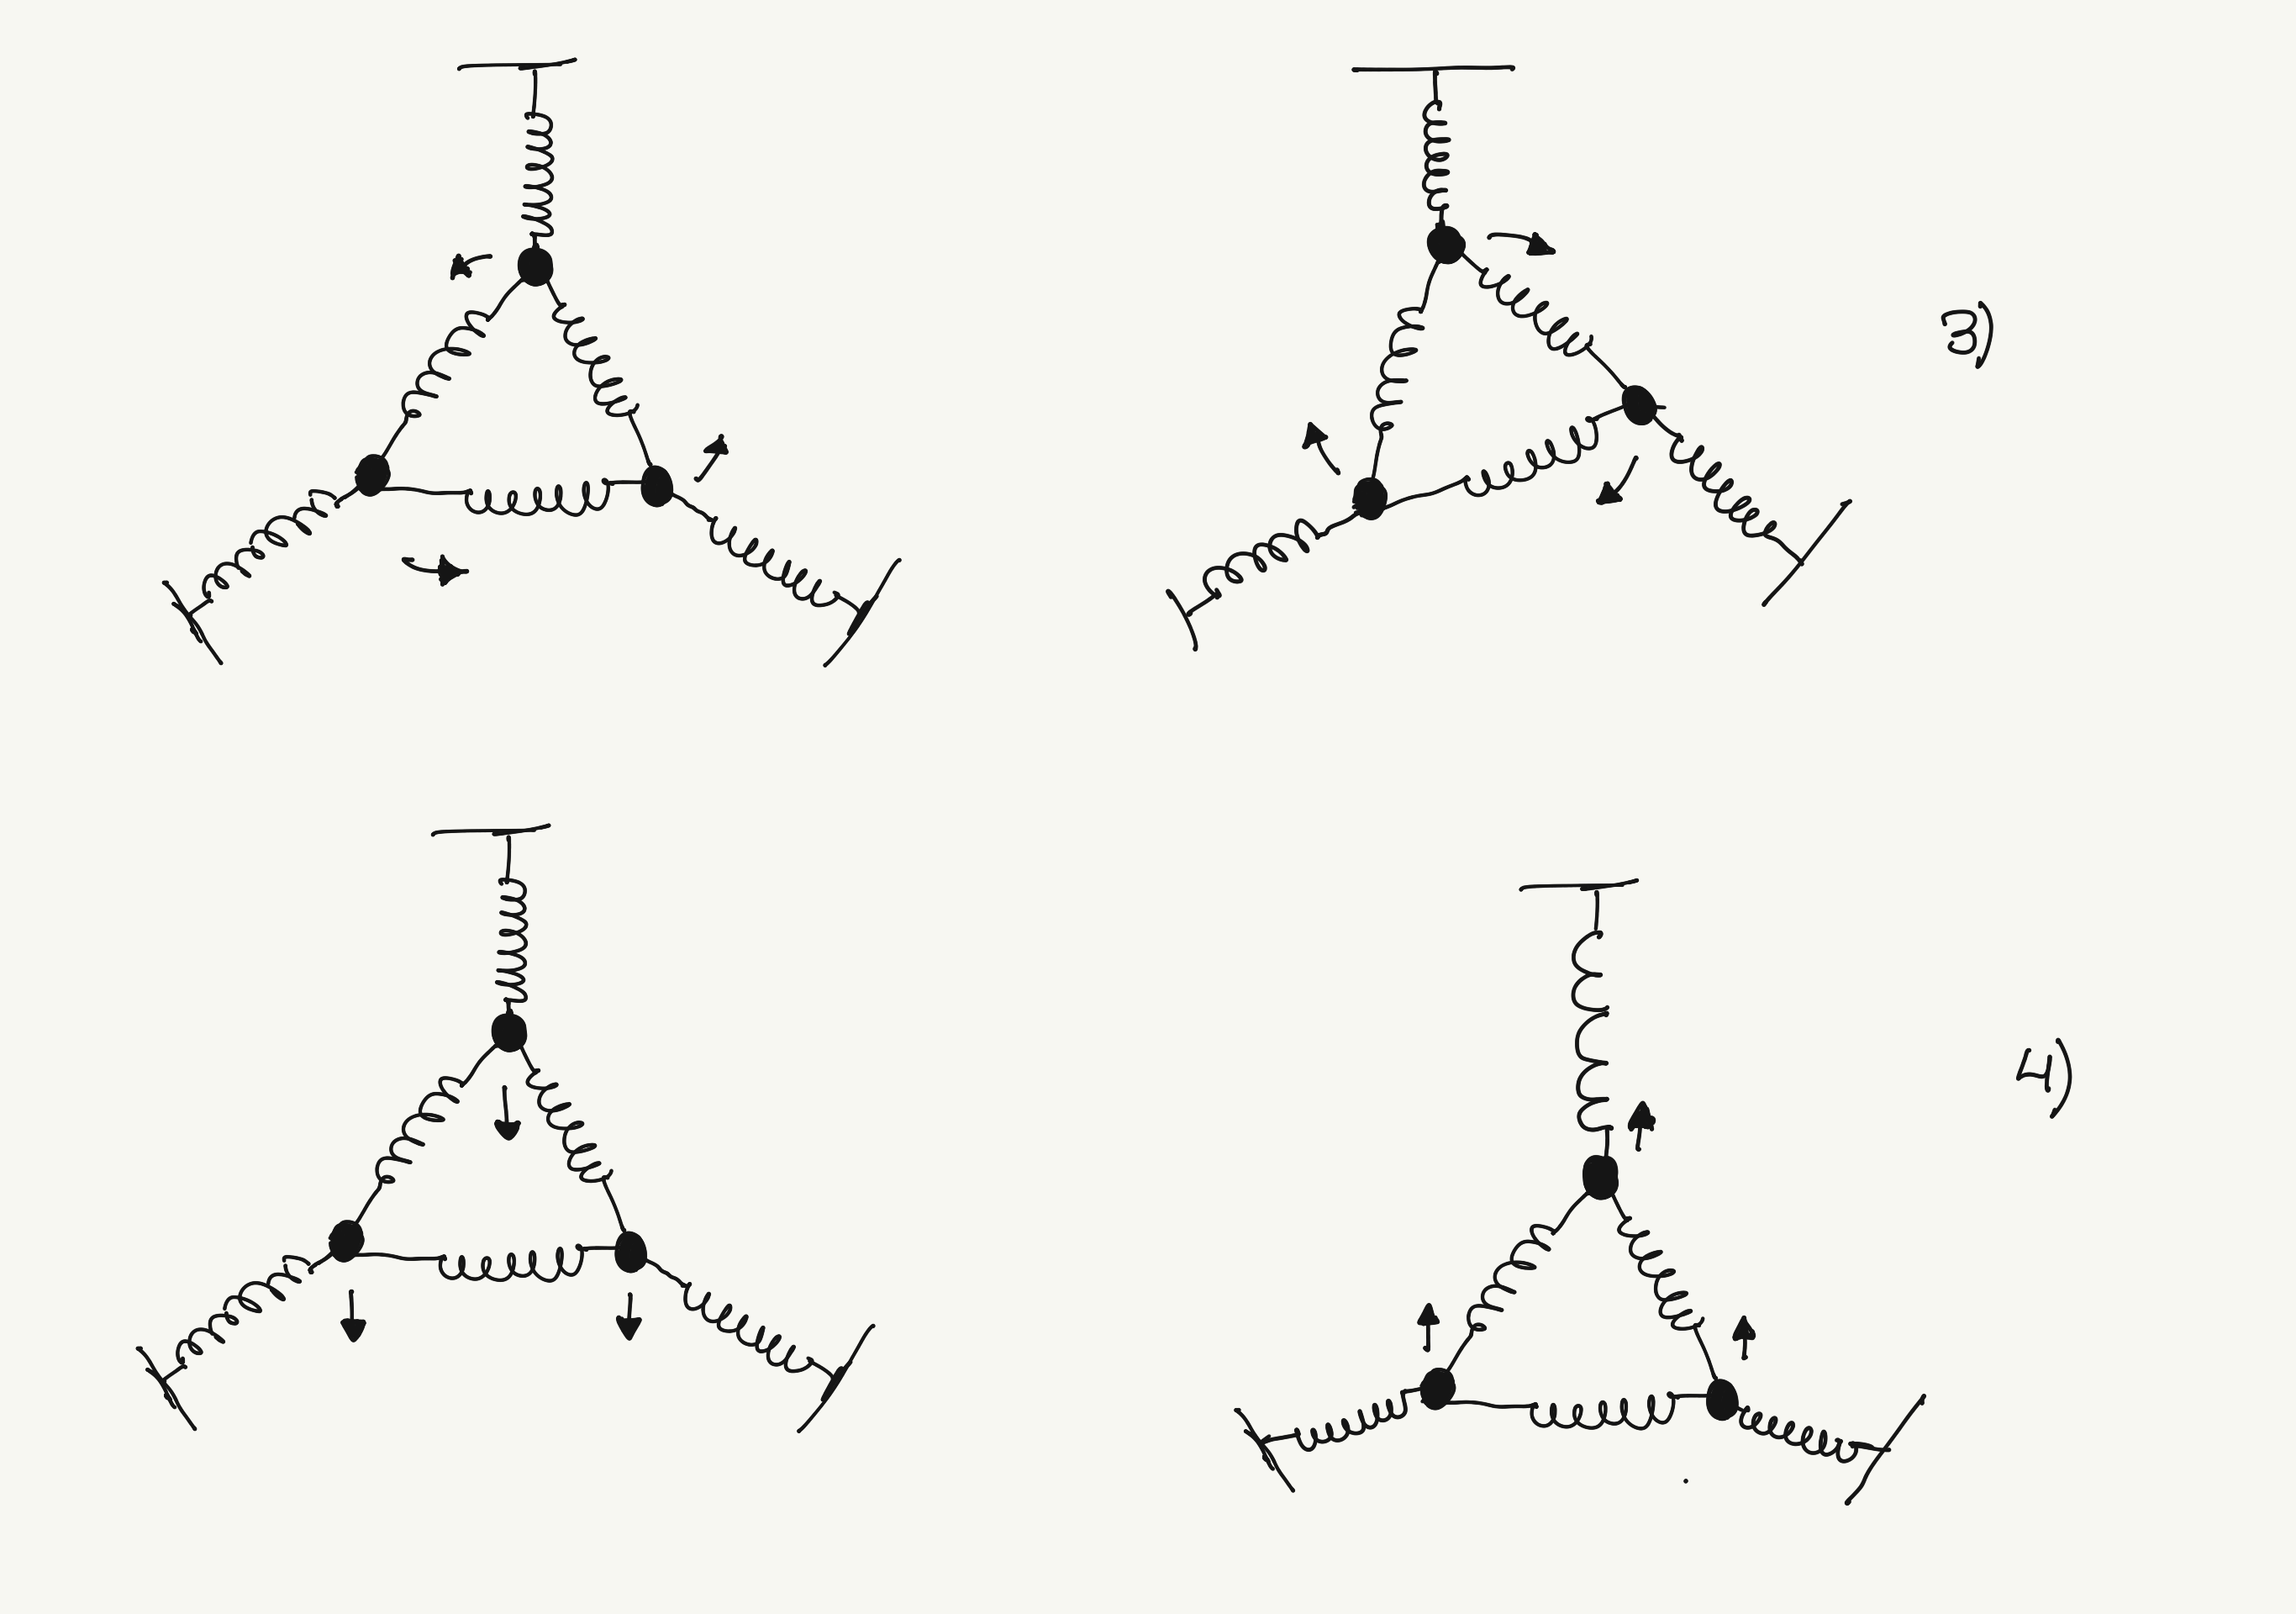
\includegraphics[scale=0.3]{Modo-normal-3.png}
\label{fig:2}
\end{figure}

Cada una de estas frecuencias normales tiene una frecuencia asociada:




\begin{table}[h!] \centering 
\begin{tabular}{|c|c|c|c|}  
\hline
  1) & 2) & 3) & 4) \\
\hline
  1.700 & 1.565 & 1.340 & 0.820 \\
\hline
\end{tabular} 
\caption{frecuencias (hz) para cada modo normal. Muelles $k_1$.}
\label{tab:7} 
\end{table}


\section{Conclusión}

Una vez obtenemos estos datos y figuras podemos concluír la práctica, ya que hemos cumplido todos los objetivos que nos propusimos, calculando las constantes de los muelles, estudiando los modos normales con 2 y 3 masas acopladas. Sin embargo antes de acabar la práctica vamos a realizar algunos comentarios adicionales sobre cada una de las partes. \\

En el cálculo de los muelles no hubo ningún tipo de problema ni nada llamativo, ya que el cálculo de constantes de recuperación del muelle ya lo hemos realizado con anterioridad en otras prácticas. Lo único que merece quizá una mención es que en la parte de cálculo de manera dinámica, tomamos varios valores de T para cada masa. Entonces lo que hacemos es hacer una media ponderada de los valores de T para una masa en concreto, y luego con esos valores ya hacemos la regresión lineal. \\

En la segunda parte no hay mucho que destacar tampoco. En general los datos teóricos coinciden bastante con los experimentales menos en la tabla \ref{tab:7} en la que podemos ver que hay una discrepancia bastante grande. Las razones por las que pudo pasar esto puede tener muchas diversas razones: quizás cometimos un fallo al medir las amplitudes, ya que si dejabas que pasara mucho tiempo se reducían, o quizás fue al medir con la regla. Para solucionarlo podríamos volver a calcularlo, para ver si el error viene dado por un fallo sistemático o realmente la amplitud teórica no coincide con la experimental para masas diferentes.  \\

En la tercera parte si que hay bastante mas que comentar. Previamente hemos dicho que debería haber 6 modos normales, pero en las figuras \ref{fig:1} y \ref{fig:2} solo se pueden ver 4 modos normales. ¿A que se puede deber esto? Pues bien, lo que ocurre es que los modos normales son degenerados. Es mucho mas sencillo de ver en el propio laboratorio, pero lo que ocurre es que por simetría debe haber un modo de estos para cada pareja (en el caso de 2)) y dos movimientos mas relativos en la dirección de uno de los muelles (en el 4)). ¡Pero esto implicaría que haya 8 modos! También tiene su explicación: como estamos en modos bidimensionales en realidad con 2 modos normales podemos construir el tercer modo normal, ya que es una base del espacio. Es decir podemos realizar una combinación lineal de los dos modos normales para obtener el tercero. \\

Una vez dicho todo esto podemos dar por concluida la práctica.

\end{document}